\documentclass[a4paper,12pt]{article}
\usepackage[utf8]{inputenc}
\usepackage[english]{babel}
\usepackage{amsmath,amssymb}
\usepackage{geometry}\geometry{margin=2.5cm}
\usepackage{enumitem}
\usepackage{booktabs}
\usepackage{tikz}
\usetikzlibrary{arrows.meta, positioning, calc, decorations.pathreplacing}
\usepackage{pgfplots}\pgfplotsset{compat=1.18}
\usepackage{tcolorbox}
\tcbuselibrary{breakable}
\usepackage{xcolor}

\newtcolorbox{merkbox}[1][]{colback=blue!5, colframe=blue!40, fonttitle=\bfseries, title={Remember}, breakable, #1}
\newtcolorbox{analogie}[1][]{colback=green!5, colframe=green!40, fonttitle=\bfseries, title={Analogy}, breakable, #1}
\newtcolorbox{begriffe}[1][]{colback=yellow!10, colframe=yellow!60!black, fonttitle=\bfseries, title={What do the terms mean?}, breakable, #1}

\title{Explanation -- HW11: Eigenvalues, Eigenvectors \& Eigenspaces}
\author{}
\date{}

\begin{document}
\maketitle

%=============================================================================
\part*{Part 1: Foundations -- explained simply}

%-----------------------------------------------------------------------------
\section*{1. What is an eigenvector? ``The direction that stays''}

A matrix $A$ is a \textbf{deformation of space}: it takes a vector and makes a new one out of it. Usually the vector is \emph{rotated and stretched} in the process. But there are special directions that are \textbf{only stretched} during the deformation -- afterwards they point exactly where they did before. These directions are the \textbf{eigenvectors}, and the stretch factor is the \textbf{eigenvalue} $\lambda$.

\begin{center}
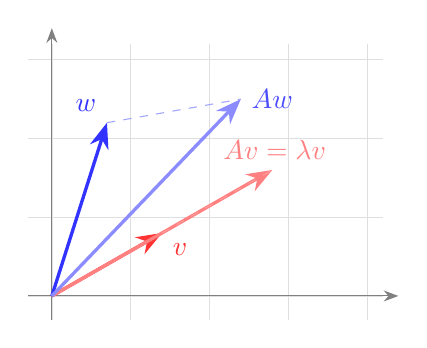
\begin{tikzpicture}[scale=1.0, >={Stealth[scale=1.1]}]
\draw[help lines, gray!25] (-0.3,-0.3) grid (4.2,3.2);
\draw[->, gray] (-0.3,0) -- (4.4,0); \draw[->, gray] (0,-0.3) -- (0,3.4);
\draw[->, red!80, very thick] (0,0) -- (1.4,0.8) node[below right, red!80]{$v$};
\draw[->, red!50, very thick] (0,0) -- (2.8,1.6) node[above]{\,$Av = \lambda v$};
\draw[red!40, dashed] (1.4,0.8) -- (2.8,1.6);
\draw[->, blue!80, very thick] (0,0) -- (0.7,2.2) node[above left, blue!80]{$w$};
\draw[->, blue!45, very thick] (0,0) -- (2.4,2.5) node[right, blue!70]{$Aw$};
\draw[blue!35, dashed] (0.7,2.2) -- (2.4,2.5);
\end{tikzpicture}
\end{center}

\begin{analogie}
Imagine a \textbf{dough} that you pull apart. A little arrow drawn on it at a slant usually rotates as you pull. But an arrow pointing exactly in the pulling direction keeps its direction -- it only gets longer. That is exactly an eigenvector, and ``how much longer'' is the eigenvalue.
\end{analogie}

\begin{merkbox}
$v \neq 0$ is an \textbf{eigenvector} of $A$ for the \textbf{eigenvalue} $\lambda$ if
\[
A v = \lambda v.
\]
The zero vector never counts as an eigenvector (otherwise everything would be trivial).
\end{merkbox}

%-----------------------------------------------------------------------------
\section*{2. How do you find the eigenvalues? The characteristic polynomial}

We rewrite $Av = \lambda v$: $Av - \lambda v = 0$, i.e.\ $(A - \lambda I)v = 0$. We are looking for a $v \neq 0$ that solves this equation. But a homogeneous system has a solution $\neq 0$ \emph{only if} the matrix $A - \lambda I$ is \textbf{not invertible} -- and that means $\det(A - \lambda I) = 0$.

\begin{merkbox}[title={The key}]
\[
\lambda \text{ is an eigenvalue} \;\Longleftrightarrow\; \det(A - \lambda I) = 0.
\]
You compute $\chi_A(t) = \det(A - tI)$ (the \textbf{characteristic polynomial}) and look for its roots.
\end{merkbox}

\begin{analogie}
$\det$ measures whether a matrix ``squashes'' directions flat. $\det(A - \lambda I) = 0$ means: $A - \lambda I$ squashes at least one direction down to $0$. Exactly that direction $v$ survives as an eigenvector, because $(A - \lambda I)v = 0$ means $Av = \lambda v$.
\end{analogie}

%-----------------------------------------------------------------------------
\section*{3. Tool A: The Sarrus rule (determinant of a $3\times3$)}

For a $3\times3$ matrix you compute the determinant with Sarrus: write the first two columns again on the right, multiply the three diagonals going \emph{down} ($+$) and subtract the three diagonals going \emph{up} ($-$).

\begin{center}
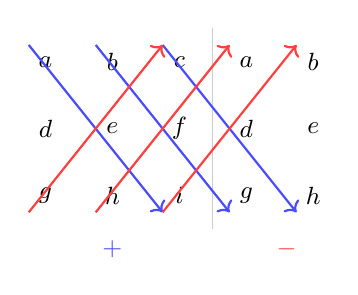
\begin{tikzpicture}[scale=0.85, every node/.style={font=\small}]
\foreach \x/\lab in {0/a,1/b,2/c,3/a,4/b} { \node at (\x,2) {$\lab$}; }
\foreach \x/\lab in {0/d,1/e,2/f,3/d,4/e} { \node at (\x,1) {$\lab$}; }
\foreach \x/\lab in {0/g,1/h,2/i,3/g,4/h} { \node at (\x,0) {$\lab$}; }
\draw[gray!40] (2.5,-0.5) -- (2.5,2.5);
\foreach \sx in {0,1,2} { \draw[->, blue!70, thick] (\sx-0.25,2.25) -- (\sx+1.75,-0.25); }
\foreach \sx in {0,1,2} { \draw[->, red!75, thick] (\sx-0.25,-0.25) -- (\sx+1.75,2.25); }
\node[blue!70] at (1.0,-0.8) {$+$}; \node[red!75] at (3.6,-0.8) {$-$};
\end{tikzpicture}
\end{center}

\begin{merkbox}[title={Sarrus formula}]
\[
\det = \underbrace{aei + bfg + cdh}_{\text{downward }(+)} - \underbrace{(ceg + afh + bdi)}_{\text{upward }(-)}.
\]
\end{merkbox}

%-----------------------------------------------------------------------------
\section*{4. Tool B: Guessing integer roots}

Once the polynomial is multiplied out (e.g.\ $t^3 - 11t^2 + 39t - 45$), you have to factor it. Trick: \textbf{integer roots are always divisors of the constant term.} For $-45$ that means $\pm1, \pm3, \pm5, \pm9, \pm15, \pm45$. You substitute them one after another until $0$ comes out.

\begin{merkbox}[title={Two free checks}]
\begin{itemize}[leftmargin=*, nosep]
    \item Sum of all eigenvalues $= \operatorname{trace}(A)$ (sum of the diagonal).
    \item Product of all eigenvalues $= \det(A)$.
\end{itemize}
This often gives you the last root without computing.
\end{merkbox}

%-----------------------------------------------------------------------------
\section*{5. Tool C: Factor out early (the elegant way)}

Instead of multiplying everything out first, you can often \emph{simplify} $\det(A - tI)$ before computing. If, for instance, \textbf{every column of $A$ has the same sum $s$}, then in $A - tI$ every column sums to $s - t$. If you add all rows into the first ($R_1 \to R_1 + R_2 + \dots$), the first row becomes all $(s-t)$ -- and $(s-t)$ can be pulled out as a factor. This immediately gives an eigenvalue $\lambda = s$ and makes the rest small.

\begin{analogie}
This is like cancelling \emph{before} multiplying out: you don't compute $\frac{6\cdot 7}{6}$ either, you cancel the $6$ first. In the same way you pull out the factor $(s-t)$ before the computation gets big.
\end{analogie}

%-----------------------------------------------------------------------------
\section*{6. Eigenspace, AM and GM}

Once you have an eigenvalue $\lambda$, you solve $(A - \lambda I)v = 0$ with Gauss. All solutions together form the \textbf{eigenspace} $E_\lambda$.

\begin{merkbox}[title={Two multiplicities -- don't mix them up!}]
\begin{itemize}[leftmargin=*, nosep]
    \item \textbf{AM($\lambda$)} (algebraic): how often $(t - \lambda)$ sits in the char.\ polynomial. \emph{(From the polynomial.)}
    \item \textbf{GM($\lambda$)} (geometric): $\dim E_\lambda$ $=$ number of free variables when solving $(A - \lambda I)v = 0$. \emph{(From the Gauss.)}
    \item It always holds that $\;1 \le \text{GM}(\lambda) \le \text{AM}(\lambda)$.
\end{itemize}
\end{merkbox}

\begin{center}
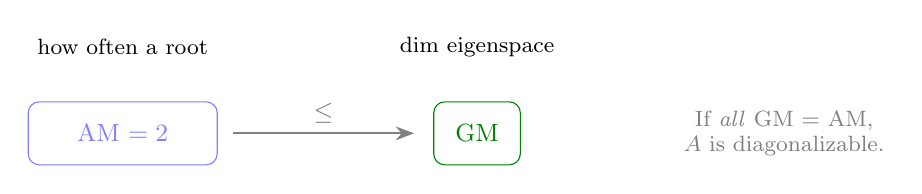
\begin{tikzpicture}[scale=1.0, every node/.style={font=\small}, >={Stealth[scale=1.0]}]
\node[draw, blue!50, rounded corners, minimum width=2.4cm, minimum height=0.8cm] (am) at (0,0) {AM $=2$};
\node[align=center] at (0,1.1) {\footnotesize how often a root};
\node[draw, green!50!black, rounded corners, minimum width=1.1cm, minimum height=0.8cm] (gm) at (4.5,0) {GM};
\node[align=center] at (4.5,1.1) {\footnotesize $\dim$ eigenspace};
\draw[->, gray, thick] (1.4,0) -- (3.7,0) node[midway, above]{$\le$};
\node[gray, align=center] at (8.4,0) {\footnotesize If \emph{all} GM $=$ AM,\\[-2pt] \footnotesize $A$ is diagonalizable.};
\end{tikzpicture}
\end{center}

\begin{analogie}
AM is \textbf{how many seats} an eigenvalue has ``reserved''; GM is \textbf{how many it actually fills with its own directions}. Filling more than reserved is impossible ($\text{GM} \le \text{AM}$). Only if every eigenvalue fills all its seats do you have enough eigenvectors for a whole basis -- then $A$ is \textbf{diagonalizable}.
\end{analogie}

%-----------------------------------------------------------------------------
\section*{7. Tool D: Eigenvalues without a polynomial (for Exercise 44)}

Sometimes you can read eigenvalues off directly, without computing:

\begin{merkbox}[title={Useful propositions}]
\begin{itemize}[leftmargin=*, nosep]
    \item $A$ \textbf{not invertible} ($\det A = 0$) $\Leftrightarrow$ $0$ is an eigenvalue. (GM$(0) = \dim\ker A$.)
    \item If a column $j$ appears as $\lambda \cdot e_j$ (just one entry $\lambda$ on the diagonal, rest $0$), then $e_j$ is an eigenvector for $\lambda$.
    \item \textbf{Rank-$1$ matrix} (all rows multiples of the same row): the eigenvalues are $\operatorname{trace}$ (once) and $0$ (otherwise).
    \item Sum of eigenvalues $= \operatorname{trace}$, product $= \det$ -- use this to fill gaps.
\end{itemize}
\end{merkbox}

\newpage

%=============================================================================
\part*{Part 2: Overview of the exercises}

\section*{Exercise 43 -- char.\ polynomial in two ways}

Two $3\times3$ matrices, the full program each. The exercise explicitly demands \textbf{both ways}:
\begin{itemize}[leftmargin=*, nosep]
    \item \textbf{Method 1:} Sarrus $\to$ multiplied-out polynomial $\to$ guess integer roots (divisors of the constant term) $\to$ factor.
    \item \textbf{Method 2:} column sums are constant ($5$ for $A$, $4$ for $B$) $\Rightarrow$ pull out the factor $(s-t)$ early, the rest to triangular form with column operations.
\end{itemize}
Then solve $(A - \lambda I)v = 0$ per eigenvalue. \textbf{Punchline:} $A$ is diagonalizable (all GM $=$ AM), $B$ is \emph{not} -- for $B$ the eigenvalue $\lambda = 2$ has AM $2$ but only GM $1$.

\section*{Exercise 44 -- eigenvalues without a polynomial}

Here the char.\ polynomial is \textbf{forbidden}; you argue with properties.
\begin{itemize}[leftmargin=*, nosep]
    \item \textbf{$A$:} row $1 =$ row $3$ $\Rightarrow$ singular $\Rightarrow$ $\lambda = 0$. Middle column $(0,6,0) \Rightarrow e_2$ is an eigenvector for $6$. The rank of $A - 6I$ is $1$, so GM$(6) = 2$; the trace $12$ confirms $0 + 6 + 6$.
    \item \textbf{$B$:} all rows multiples of $(1,1,1,1)$ $\Rightarrow$ rank $1$ $\Rightarrow$ GM$(0) = 3$. Trace $= 5+7+11-23 = 0 \Rightarrow$ there is no further eigenvalue $\Rightarrow$ $\lambda = 0$ with AM $4$. Because GM $3 <$ AM $4$, it is \emph{not} diagonalizable.
\end{itemize}

\section*{Exercise 45 -- four short proofs}

Always the same pattern: take $v \neq 0$ with $Av = \lambda v$ and check that $v$ is also an eigenvector of the new matrix.
\begin{itemize}[leftmargin=*, nosep]
    \item \textbf{(a)} $(A + cI)v = \lambda v + cv = (\lambda + c)v$.
    \item \textbf{(b)} $A^2 v = A(\lambda v) = \lambda^2 v$.
    \item \textbf{(c)} For invertible $A$, $\lambda \neq 0$; from $Av = \lambda v$ it follows that $A^{-1}v = \tfrac1\lambda v$.
    \item \textbf{(d)} $(AB)v = A(\mu v) = \lambda\mu\, v$ (if $Av = \lambda v$, $Bv = \mu v$).
\end{itemize}

%=============================================================================
\section*{Summary}

\begin{center}
\begin{tabular}{@{}lll@{}}
\toprule
Matrix & Eigenvalues (AM, GM) & diagonalizable? \\
\midrule
$43\,A$ & $3\,(2,2)$, \; $5\,(1,1)$ & yes \\
$43\,B$ & $2\,(2,1)$, \; $4\,(1,1)$ & no \\
$44\,A$ & $0\,(1,1)$, \; $6\,(2,2)$ & yes \\
$44\,B$ & $0\,(4,3)$ & no \\
\bottomrule
\end{tabular}
\end{center}

\begin{merkbox}[title={Golden rules}]
\begin{enumerate}[leftmargin=*, nosep]
    \item Eigenvalues $=$ roots of $\det(A - tI)$.
    \item Trace $=$ sum of eigenvalues, $\det =$ product -- always use as a check.
    \item Constant column sums $s$ $\Rightarrow$ factor $(s-t)$ and eigenvalue $s$ for free.
    \item $\det = 0 \Leftrightarrow 0$ is an eigenvalue; rank-$1$ matrix $\Rightarrow$ eigenvalues $\operatorname{trace}$ and $0$.
    \item Per eigenvalue: solve $(A - \lambda I)v = 0$ $\to$ basis $\to$ GM $=$ number of free variables.
    \item All GM $=$ AM $\Rightarrow$ diagonalizable.
\end{enumerate}
\end{merkbox}

\end{document}
